\scanpage{49}
Reste à traiter le cas (très particulier !) où
$\nexists$ ps. droite $\Delta$ qui ne passe par $s$ ni par $s'$.
\inserted{Soit $\Theta$ la ps. droite déterminée par $a$,}
Considérons alors une ps. droite $D$ \inserted{$\ne\Theta$} passant par
$s$, \deleted{\unsure{soit}} une $D'$ \inserted{$\ne\Theta$} passant par $s'$,
\deleted{\unsure{on|soit}} a donc $D\ne D'$, soit
$t$ l'intersection de $D$ et $D'$.
Soit, \deleted{\unsure{$b$ une des deux|$b$ une des|$b$ un des deux}} \inserted{$K'={}$} $K_{\{\Theta,D,D'\}}$,
\figure{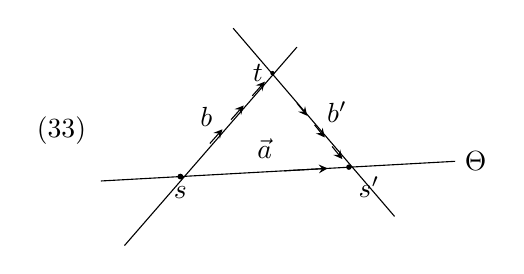
\begin{tikzpicture}[>=stealth]
\draw (-2.15,-.12)--(2.35,.13) node[right] {$\Theta$};
\draw (-1.85,-.94)--(.34,1.58); \draw (-.47,1.82)--(1.58,-.57);
\coordinate (s) at (-1.14,-.064); \coordinate (t) at (.03,1.25); \coordinate (h) at (1.0,.056);
\fill (s) circle (.037) node[below] {$s$}; \fill (t) circle (.028) node[left] {$t$}; \fill (h) circle (.035) node[below right] {$s'$};
\foreach \p in {.32,.55,.78}{\draw[->] ({-1.14+1.17*\p},{-.064+1.314*\p})--++(.16,.18);
\draw[->] ({.03+.97*\p},{1.25-1.194*\p})--++(.13,-.16);}
\draw[->] (.18,.009)--(.73,.04); \node[above] at (-.07,.04) {$\vec a$}; \node[left] at (-.61,.70) {$b$}; \node[right] at (.60,.75) {$b'$}; \node at (-2.65,.52) {(33)};
\end{tikzpicture}}
$b$ une des arêtes qui joignent $s$ à $t$, et prenons
l'unique arête $b'$ de $\unsure{\widetilde K'|K'}$ qui joigne $t$ à $s'$, et
telle que $\{a,b,b'\}$ soit compatible avec l'
orientation de $K'$. Alors $b$ et $b'$ ne sont pas
nécessairement des arêtes de $K$, mais ils
se décomposent en succession d'arêtes de $K$.
% slanted
\margin{$\Downarrow$ Autre méthode, plus simple : On note que $\unsure{\vec v_{\vec a}|\vec u_{\vec a}|\vec\psi_{\vec a}}:\vec{\unsure{Z|\mathcal Z|\mathfrak Z}}_s\mathbin{-}\vec Z_{s'}$ est connu, quand on connaît, pour un ordre circulaire $\in\vec Z_s$, la restriction de l'ordre associé sur \deleted{\unsure{la partie}} la partie de $\vec I_{s'}$ définie par deux droites $\Theta,D'$\ldots}

On suppose que $K$ n'est pas \inserted{réduit à} une \deleted{sécante}
famille, de \inserted{$n\geq3$} ps. droites concourantes
coupées par une seule sécante (ce qui
% slanted
\margin{\uline{NB} \unsure{Obs.} que $K$ \unsure{comporte|compte} au moins 4 ps. droites (le cas de 3 \unsure{est} déjà traité !)}
signifie que les \inserted{$n$} ps. droites passant par
le sommet privilégié $s$ sont toutes des
bigônes.). Dans ce cas, la \deleted{droite}\inserted{ps. dr.} $\Theta$
est l'\uline{unique} ps. droite qui soit un bigône,
donc $D$ et $D'$ n'en sont pas, donc on
peut définir les $u_{\vec c}$ pour des arcs \inserted{de $K$} portés
par $D$, ou par $D'$. On définit alors
% archive sheet number: 48
